% !TeX spellcheck = sv_SE
\documentclass[a4paper]{IEEEtran}
\def\thepage{} %a4paper adds page numbers, this fix removes them

\usepackage[pdftex]{graphicx}
\usepackage[T1]{fontenc}
\usepackage[utf8]{inputenc} 

\usepackage[swedish]{babel}
\usepackage{url}

\usepackage{scrextend}

\hyphenation{inne-bär}

\title{Autonomous Vehicles}
% http://www.software-center.se/digitalAssets/1521/1521374_kent-sw-center---software---need-for-speed.v001.pdf
% 1. Teknisk översikt
% 2. Nutida tillämplingar
% 3. Framtida och möjliga tillämpningar
% 4. Konkurrerande teknologier och standarder. Fördelar och nackdelar
% 5. Egna slutsatser

\author{\IEEEauthorblockN{Niklas Hedström, Emil Wihlander\\ }
\IEEEauthorblockA{Lunds Tekniska Högskola\\
Lund, Sverige\\
Email: \{dat15ewi, dat15nhe\}@student.lu.se}}

%----------------------------------------------------------------

\begin{document}
\maketitle

\begin{abstract}

\end{abstract}


\section{Introduktion}
\emph{Autonomous vehicles}, eller \emph{självkörande fordon}, är fordon som på ett eller annat sätt kan styra sig själv baserat på omgivningen. 
\emph{SAE International} har definierat klassificeringsnivåer som inom industrin har blivit allmänt accepterade där fordon klassas från SAE level 0 - Ingen automatisering, till SAE level 5 - fullt automatiserad. \cite{SAE2014} 

Denna rapport kommer behandla den kommunikation som behöver ske för att självkörning ska kunna fungera, det innebär både intern och extern kommunikation. 
Det inkluderar teknologier som redan är standardiserade och välanvända samt potentiella teknologier som idag inte är färdigutvecklade men ger möjligheten att lösa problem som idag saknar en universellt använd lösning.

Huvudfokus kommer ligga på \emph{självkörande bilar} snarare fordon då det finns ett stort intresse både bland klassiska biltillverkare så som Volvo, Mercedes-Benz och Ford och nya företag inom bilbranschen så som Google, Tesla och Uber att vara först ut. \cite{VolvoAD}\cite{MercedesAD}\cite{FordAD}\cite{GoogleAD}\cite{TeslaAD}\cite{UberAD}
Den konkurrenspräglade miljön innebär att företagen har varit öppna om sina framsteg inom området och har därmed publicerat mycket information.

\section{Klassificering}
\emph{SAE international standard J3016} definierar de olika nivåerna av självkörning enligt: \cite{SAE2014}

\vspace{10 pt}
\begin{labeling}{nivå 1}
	\item [\textbf{nivå 0}] \emph{No Automation}. Fordonet saknar helt självkörning. Kan skicka varningar till föraren, men är inget krav.
	\item [\textbf{nivå 1}] \emph{Driver Assistance}. Fordonet har vissa funktioner som påverkar det baserat på omgivningen. T.ex. ACC (Adaptive Cruise Control)\footnote{När fordonet kan ändra farthållaren baserat på hastigheten av framförvarande fordon\cite{ACC}}, LKA (Lane Keeping Assistance)\footnote{När fordonet kan hjälpa till att styra så att den håller sig inom nuvarande fil\cite{LKA}} och Parkeringshjälp\footnote{När fordonet hjälper till att parkera genom att ta över styrningen\cite{AP}}. Föraren måste dock alltid vara redo att ta över.
	\item [\textbf{nivå 2}] \emph{Partial Automation}. Fordonet kan själv manövrera sig i kända förutsättningar, men när förutsättningar inte längre uppfylls måste föraren ta över genast.
	\item [\textbf{nivå 3}] \emph{Conditional Automation}. Fordonet ska utöver nivå 2 kunna hantera dynamiska situationer i specifika miljöer, så som huvudleder där gångtrafikanter saknas. Detta innebär att föraren kan släppa fokus helt i dessa miljöer.  
	\item [\textbf{nivå 4}] \emph{High Automation}. Fordonet ska utöver nivå 3 kunna hantera situationer som inte förväntas uppstå och kunna agera därefter.
	\item [\textbf{nivå 5}] \emph{Full Automation}. Fordonet ska utöver nivå 4 kunna hantera alla miljöer och därmed aldrig kräva input från en potentiell förare.
\end{labeling}

\section{Nuvarande Implementation}


\begin{figure}
	\begin{center}
		\resizebox{!}{60mm}{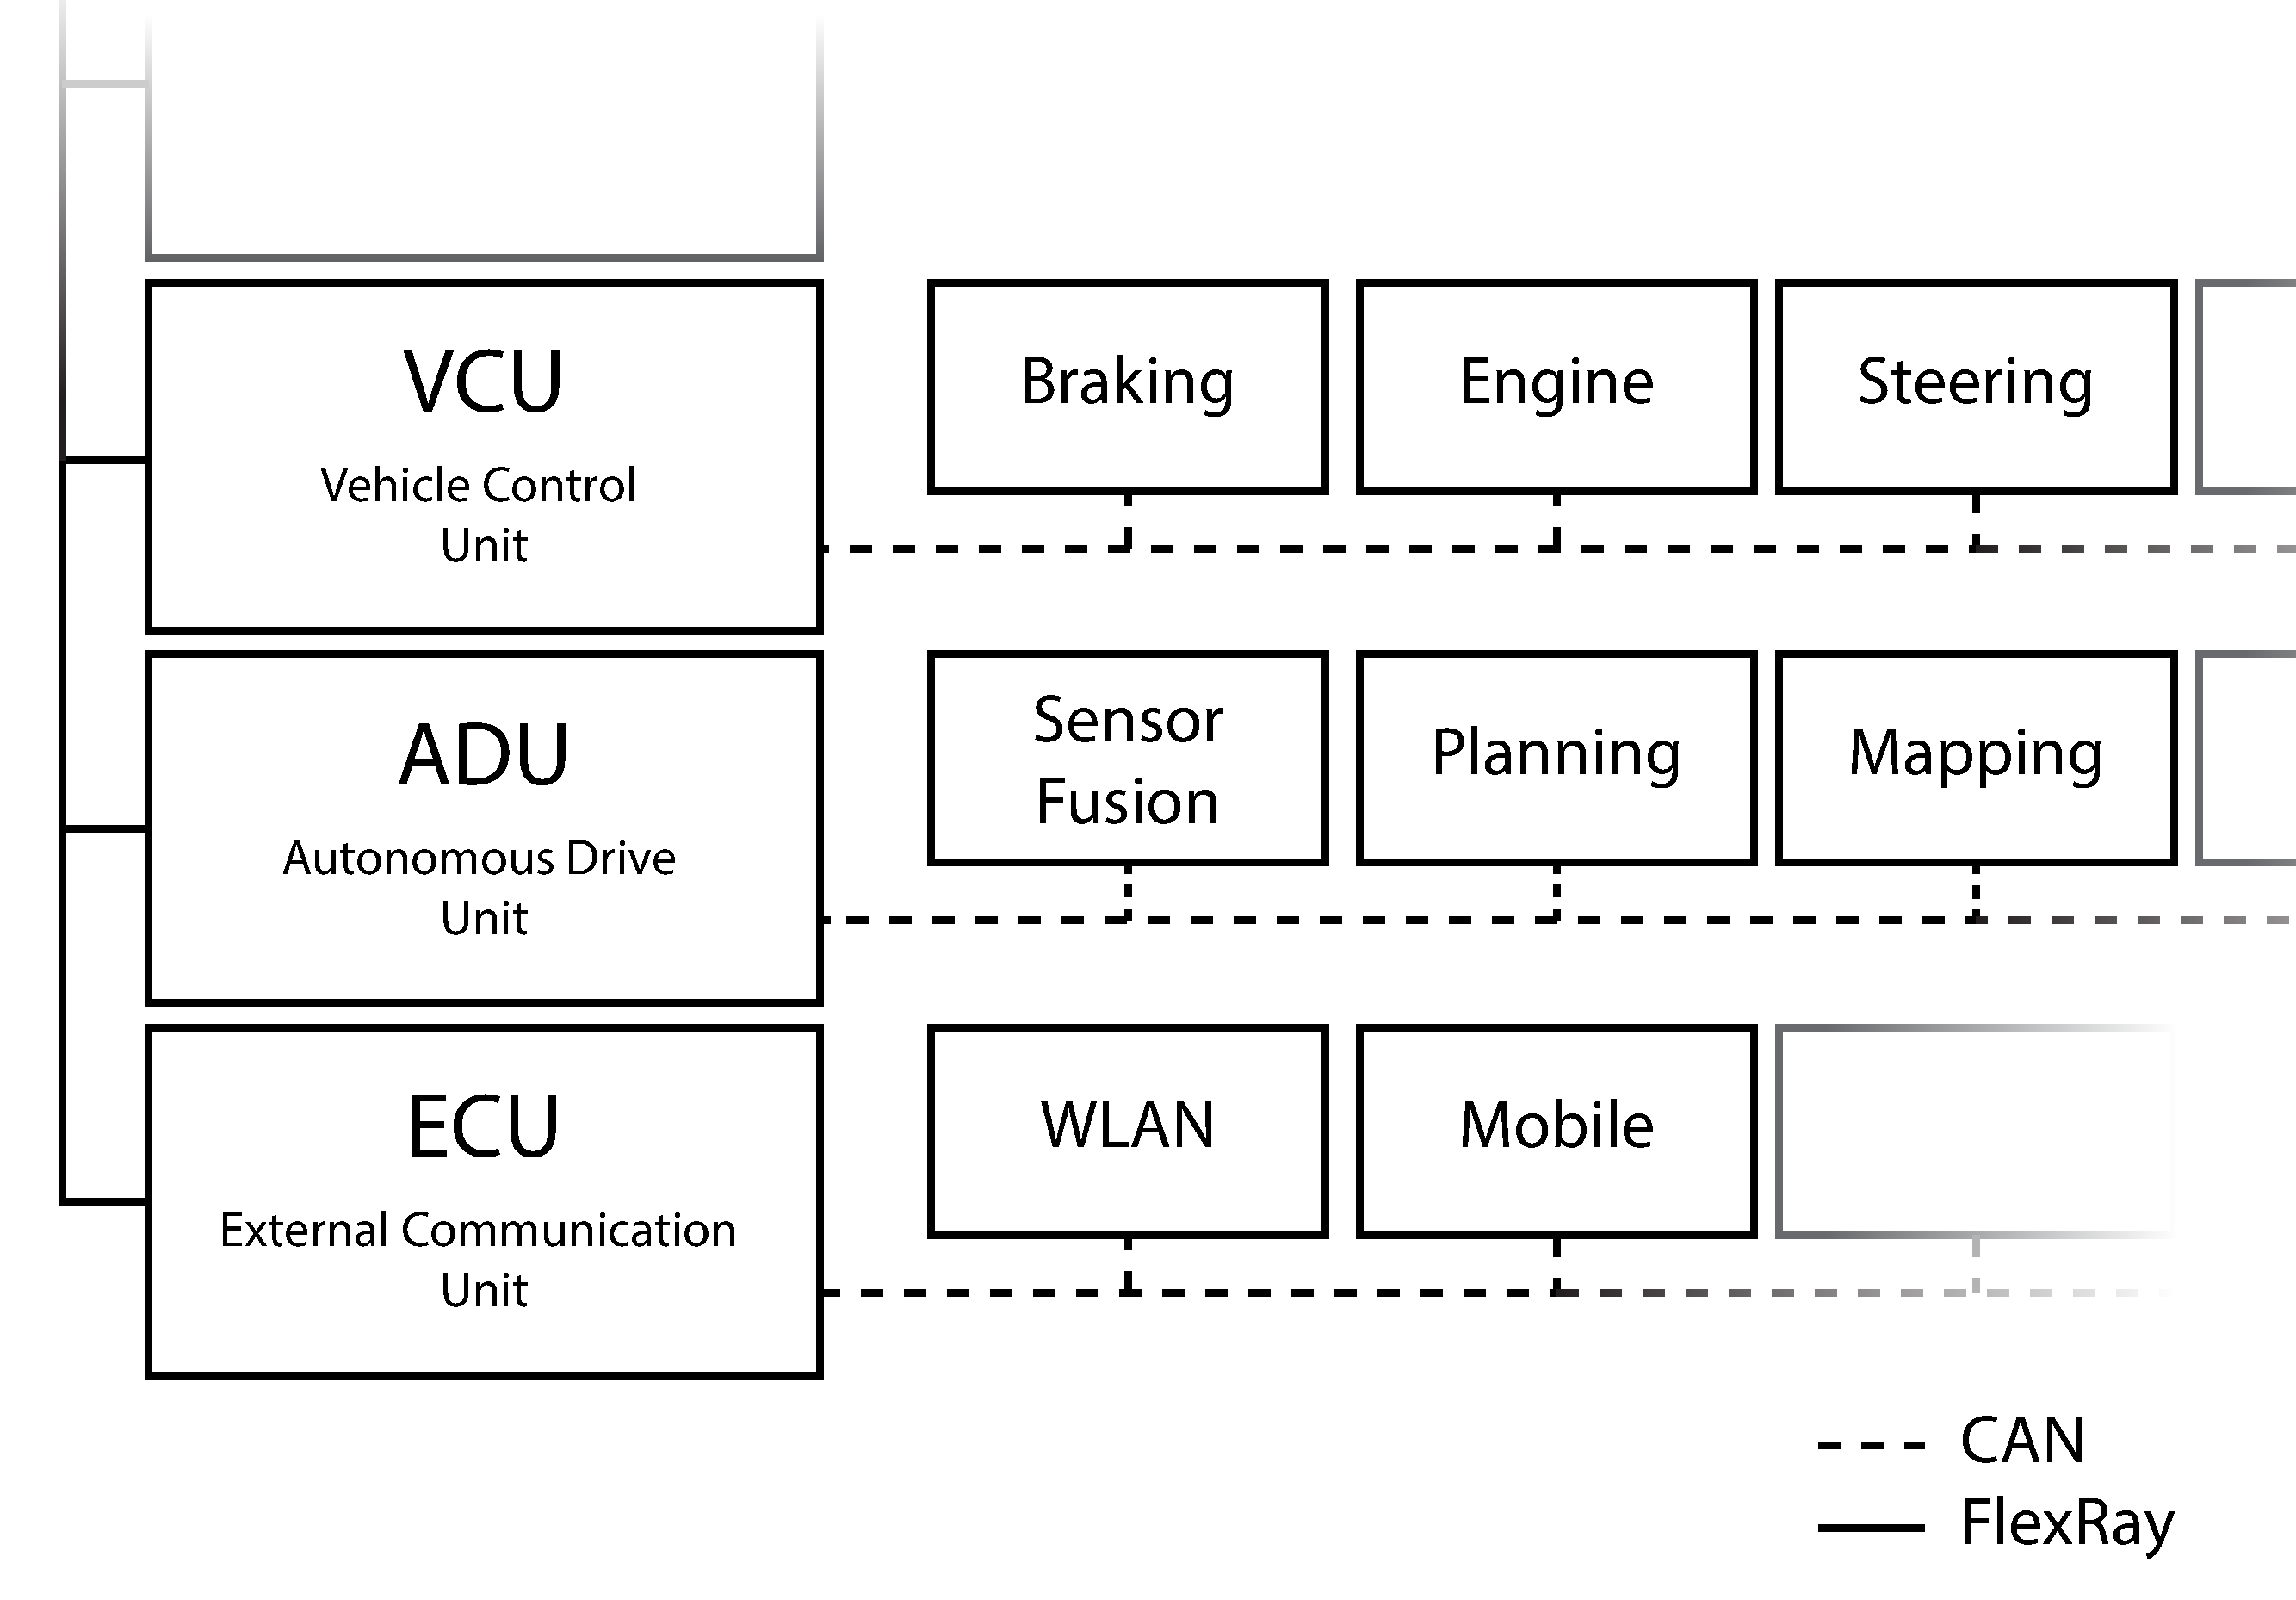
\includegraphics{CarCommunicationScheme.pdf}}
	\end{center}
	\caption{En förenklad modell över hur ett nät inuti en bil skulle kunna se ut.}
	\label{CarScheme}
\end{figure}

\section{Internal Vehicle Communication}

\subsection{Controller Area Network}

\subsubsection{Physical Layer}
Det fysiska lagret i CAN-Bussen består av tre sublager the physical coding (PCS) som är implementerat i CAN-bussens kontroll chip, the physical media attachment (PMA) som specificerar transceiverns egenskaper och the physical media-dependent sub-layers (PMS) som är programspecifik och är inte generellt standardiserad.

The physical coding sublagret i CAN-bussen använder sig av NRZ kodning, jämför med manchester kodning så behöver man inte med NRZ i varje bit ha en fallande eller stigande flank utan signalen kan hållas konstant över en längre period om de överförda bitarna har samma logiska värde. Således måste åtgärder vidtas för att försäkra sig om att det maximala tillåtna intervallet mellan två signalflanker inte överskrids. Detta är viktigt för synkroniseringen. Åtgärdens som gör är att CAN-bussen använder ett protokoll som gör att när det kommer fem bitar av samma värde lägger CAN-buss kontrollen in en bit av motsattvärde, även kallat ”bit stuffing”. Sedan gör den mottagande CAN-buss noden det motsatta och tar bort de instoppade bitarna.
Om bussen är inaktiv så används den första fallande flanken till att globalt synkronisera alla CAN-buss kontroller. 

The physical media attachment sublagret är normalt implementerat i transceiver chipet. Inputen är TxD och RxD signalerna från CAN-buss kontrollen och outputen driver busslinjerna. \cite{CANphys}

\subsubsection{Data Link Layer}

\subsection{FlexRay}

\section{External Vehicle Communication}

\subsection{Car to Car Communication}

\subsection{Cloud to Car Communication}

\section{Slutsats}








\begin{thebibliography}{77}
	\bibitem{SAE2014}SAE International: \emph{Automated Driving}, 
	
	http://www.sae.org/misc/pdfs/automated\_driving.pdf, 
	
	2014 (hämtad 2016-12-02)
	
	\bibitem{VolvoAD}Volvo: \emph{Volvo Cars presents a unique solution for integrating self-driving cars into real traffic}, 
	
	https://www.media.volvocars.com/global/en-gb/media/pressreleases/158276/volvo-cars-presents-a-unique-system-solution-for-integrating-self-driving-cars-into-real-traffic, 
	
	2015-02-19 (hämtad 2016-12-02)
	
	\bibitem{MercedesAD}Mercedes: \emph{The Mercedes-Benz F 015 Luxury in Motion.}, 
	
	https://www.mercedes-benz.com/en/mercedes-benz/innovation/research-vehicle-f-015-luxury-in-motion/ 
	
	(hämtad 2016-12-02)
	
	\bibitem{FordAD}Ford: \emph{Ford börjar testa självkörande bilar i Europa under 2017}, 
	
	http://www.mynewsdesk.com/se/ford/pressreleases/ford-boerjar-testa-sjaelvkoerande-bilar-i-europa-under-2017-1670717, 
	
	2016-11-29 (Hämtad 2016-12-02)
	
	\bibitem{GoogleAD}Google: \emph{Google Self-Driving Car Project}, 
	
	https://www.google.com/selfdrivingcar/ 
	
	(hämtad 2016-12-02)
	
	\bibitem{TeslaAD}Tesla: \emph{All Tesla Cars Being Produced Now Have Full Self-Driving Hardware}, 
	
	https://www.tesla.com/blog/all-tesla-cars-being-produced-now-have-full-self-driving-hardware, 
	
	2016-10-19 (hämtad 2016-12-02)
	
	\bibitem{UberAD}Uber: \emph{Pittsburgh, your Self-Driving Uber is arriving now}, 
	
	https://newsroom.uber.com/pittsburgh-self-driving-uber/, 
	
	2016-09-14 (hämtad 2016-12-02)
	
	\bibitem{ACC}Wikipedia: \emph{Autonomous cruise control}, 
	
	https://en.wikipedia.org/wiki/Autonomous\_cruise\_control\_system, 
	
	2016-12-01 (Hämtad 2016-12-01)
	
	\bibitem{LKA}Toyota: \emph{Lane Keeping Assist}, 
	
	http://www.toyota-global.com/innovation/safety\_technology/safety\_
	
	technology/technology\_file/active/lka.html 
	
	(Hämtad 2016-12-01)
	
	\bibitem{AP}Wikipedia: \emph{Automatic parking}, 
	
	https://en.wikipedia.org/wiki/Automatic\_parking, 
	
	2016-11-24 (Hämtad 2016-12-01)
	
	\bibitem{CANphys}CAN in Automation (CiA): \emph{CAN physical layer},
	
	https://www.can-cia.org/can-knowledge/can/systemdesign-can-physicallayer/
	
	(hämtad 2016-12-04)
%\bibitem{gsma}S. Parkvall: \emph{Broadband Wireless Access - HSPA and LTE}, http://www.s3.kth.se/signal/edu/s3\_seminar/2009/talks/sem2.pdf (last visited 2009-03-12)
%\bibitem{hostmfl} P. Ödling, T. Magesacher, M. Berg, E. A. Sanchez, S. Höst and P. Börjesson: \emph{The Fourth Generation Broadband Concept}, IEEE Communications Magazine, Vol. 47, No. 1, pp. 63-69, IEEE Communication Society, 2009
\end{thebibliography}

\end{document}
